\begin{frame}{Material e métodos}{Tratamentos térmicos - DRX \textit{in situ}}
	\begin{itemize}
		\item Energia do feixe: 12keV $\rightarrow \lambda=1,033$\AA
		\item Geometria $\omega-2\theta$; $\omega$ fixo em 15°
		\item Dois detetores multicanal Mythen 1K com 1280 pixels cada
		\item Aquisições: detetores posicionados a 31° $\rightarrow$ 26°--47° (picos (111) e (200) de $\gamma$ e (110) e (200) de $\alpha$); acq. feitas a cada 3,5s
		\item Varreduras: goniômetro varre 26° $< 2\theta$ < 86°
	\end{itemize}

	\begin{figure}
	\includegraphics[width=4.5cm]{img/acq.pdf}
	\includegraphics[width=4.5cm]{img/scan.pdf}
	\end{figure}
\end{frame}

\begin{frame}{Material e métodos}{Tratamentos térmicos - DRX \textit{in situ}}
	\begin{figure}
		\centering
		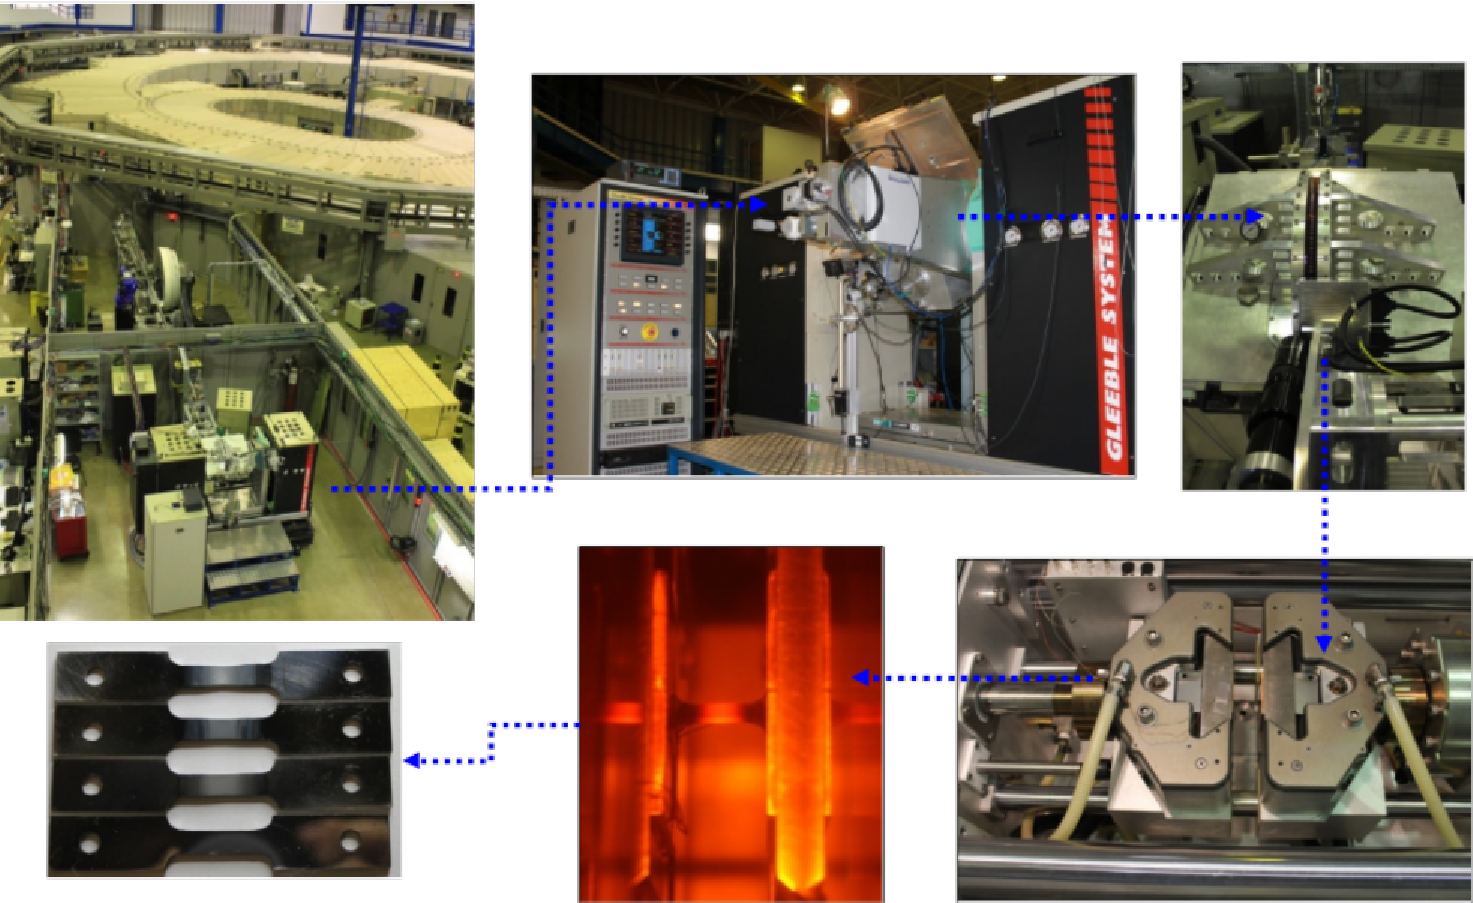
\includegraphics[width=\textwidth]{./img/XTMS_facilities.pdf}
	\end{figure}
\end{frame}
%\begin{frame}{Material e métodos}{Tratamentos térmicos - DRX \textit{in situ}}
	%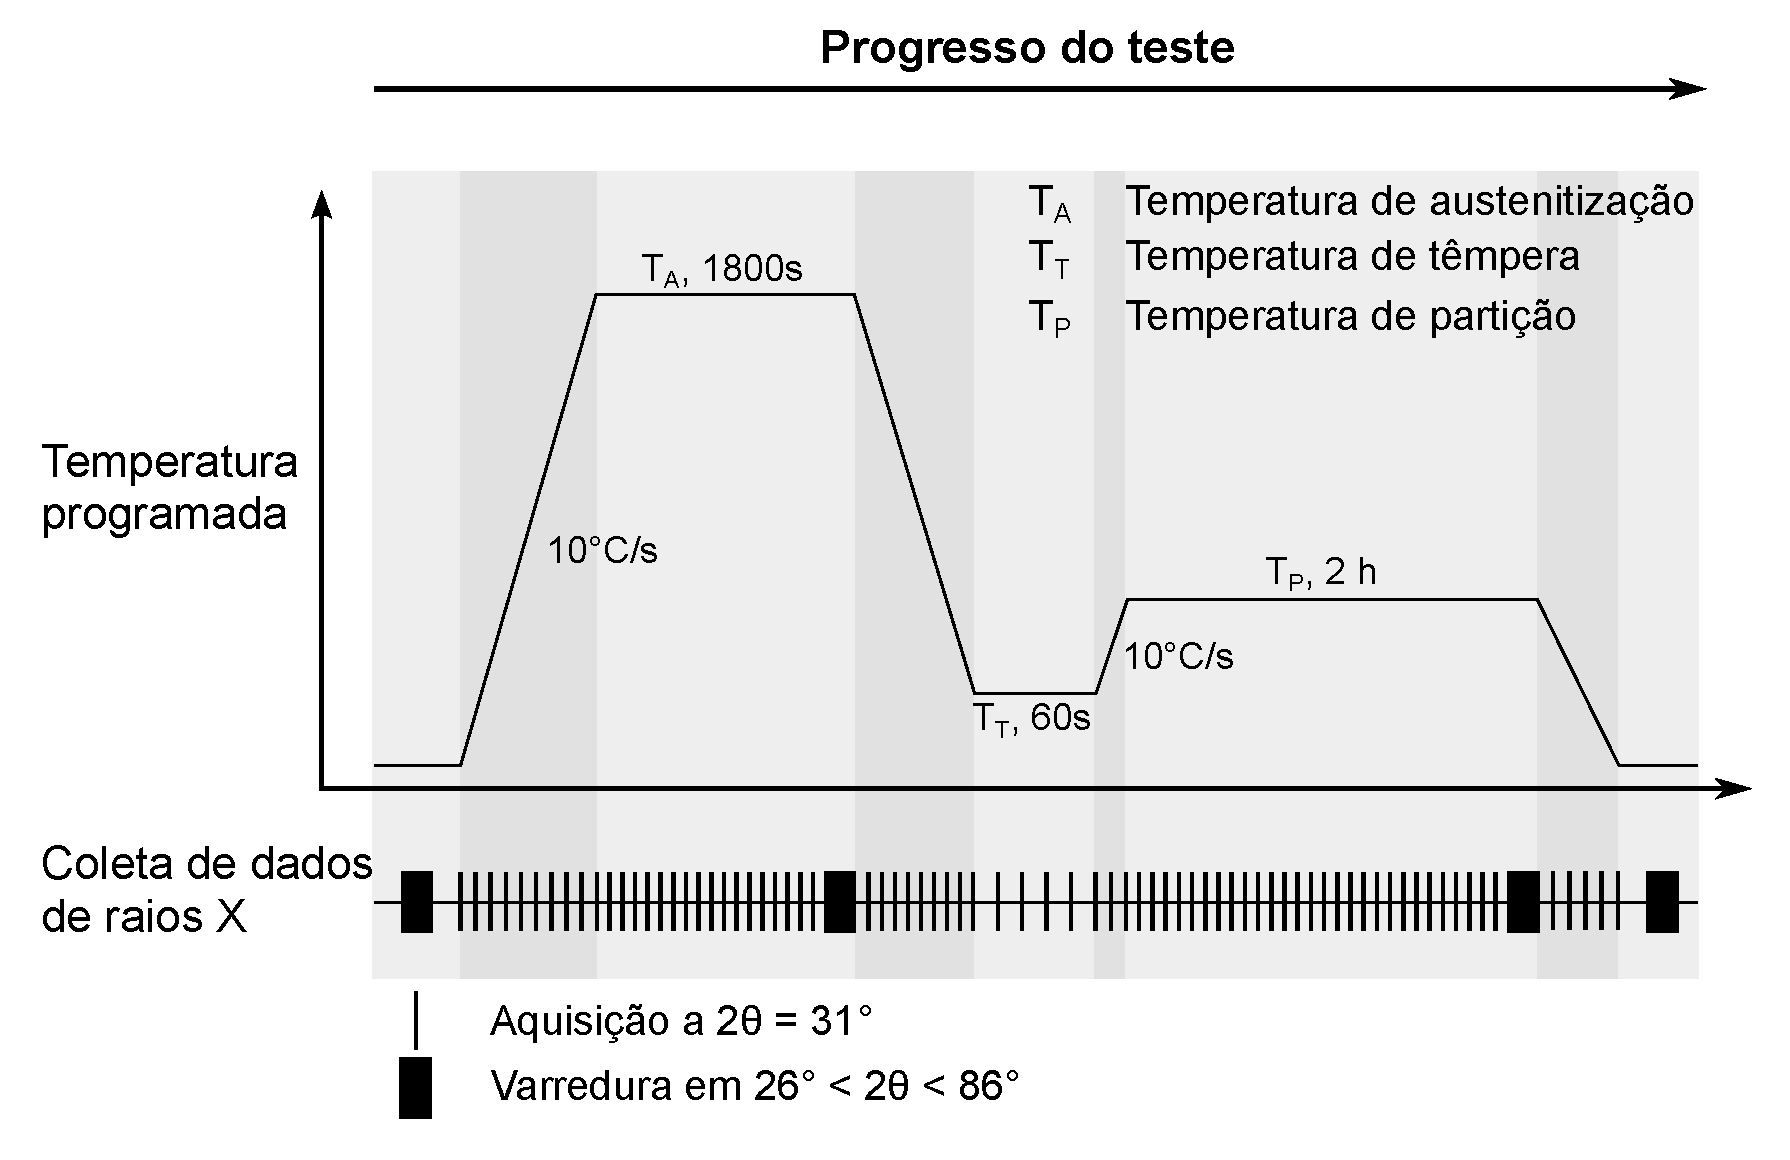
\includegraphics[width=10cm]{../texto/img/expproc_XTMS.pdf}
%\end{frame}